\chapter{Espacios de trabajo para el estudio}

\section{Entornos didácticos}\label{entornos_didacticos}

Ya se ha explicado que practicar cualquier tipo de explotación de vulnerabilidades sobre dispositivos de terceros sin consentimiento explícito, incluso si no se pretende (ni se llega a) hacer ningún daño, es ilegal y puede acarrear serios problemas legales.

Es por ello que a la hora de obtener formación especifica en este ámbito y, sobretodo, de ponerla en práctica se recomienda hacer uso de \textbf{entornos didácticos} simulados en la nube, en los que podemos `atacar' máquinas virtuales preparadas para ello y sin ningún riesgo legal o moral.

Como una parte importante del trabajo consiste en investigar sobre pentesting y hacer pruebas con herramientas típicas del mismo, hemos dedicado algo de tiempo a investigar sobre algunas plataformas interesantes para ello. Las describimos a continuación.

\begin{description}
    \item[Hackthebox] es una plataforma de hacking que aloja distintas máquinas vulnerables y tiene un planteamiento en el que los usuarios pueden acceder a esas máquinas y tratar de explotar sus vulnerabilidades para conseguir `flags' (banderas), unos códigos que demuestran que se han completado ciertos retos, como por ejemplo conseguir permisos de administrador dentro del sistema. Es especialmente interesante porque constantemente se añaden nuevas máquinas y nuevos retros, hay rankings, etc..
    \item[Tryhackme]: es una plataforma más enfocada al aprendizaje que hackthebox. En esta también se despliegan máquinas virtuales que serán `atacadas' pero estas forman parte de `salas' de aprendizaje que contienen lecciones teóricas (por escrito) e instrucciones para llevar a cabo tareas sobre las máquinas desplegadas con el objetivo de ir avanzando en la sala. Quizá tiene un carácter menos competitivo que Hackthebox y un menor nivel de `gamificación' pero es una plataforma muy didáctica y muy útil para aprender sobre pentesting.
    \item[VulnHub]: esta plataforma permite alojar máquinas virtuales vulnerables. Es mucho más simple que las otras, no hay competición ni comparativas de ningún tipo, simplemente individuos que sube sus máquinas y otras que pueden descargarlas, deplegarlas en local e intentar atacarlas. La ventaja que tiene es que permite descargar las imágenes para desplegar tú mismo las máquinas virtuales en lugar de desplegarlas en la nube.
\end{description}

Estas tres plataformas se han utilizado durante el trabajo para aprender y practicar técnicas de pentesting. En especial mencionaremos Vulnhub porque será la que se utilice durante la fase final del proyecto para un ejemplo de caso práctico de pentesting.

\section{Kali Linux y Wazuh}

\subsection{Kali Linux}

Aunque una parte importante del entorno de pruebas son aquellas máquinas cuyas vulnerabilidades vamos a tratar de explotar, la principal herramienta que usaremos en nuestro estudio será una instancia virtual de Kali Linux, una distribución de Linux de la que ya hemos hablado, que se especializa en test de penetración de sistemas y que tiene multitud de herramientas que nos servirán para llevar a cabo una auditoría.

\begin{figure}[!hbt]
  \centering
  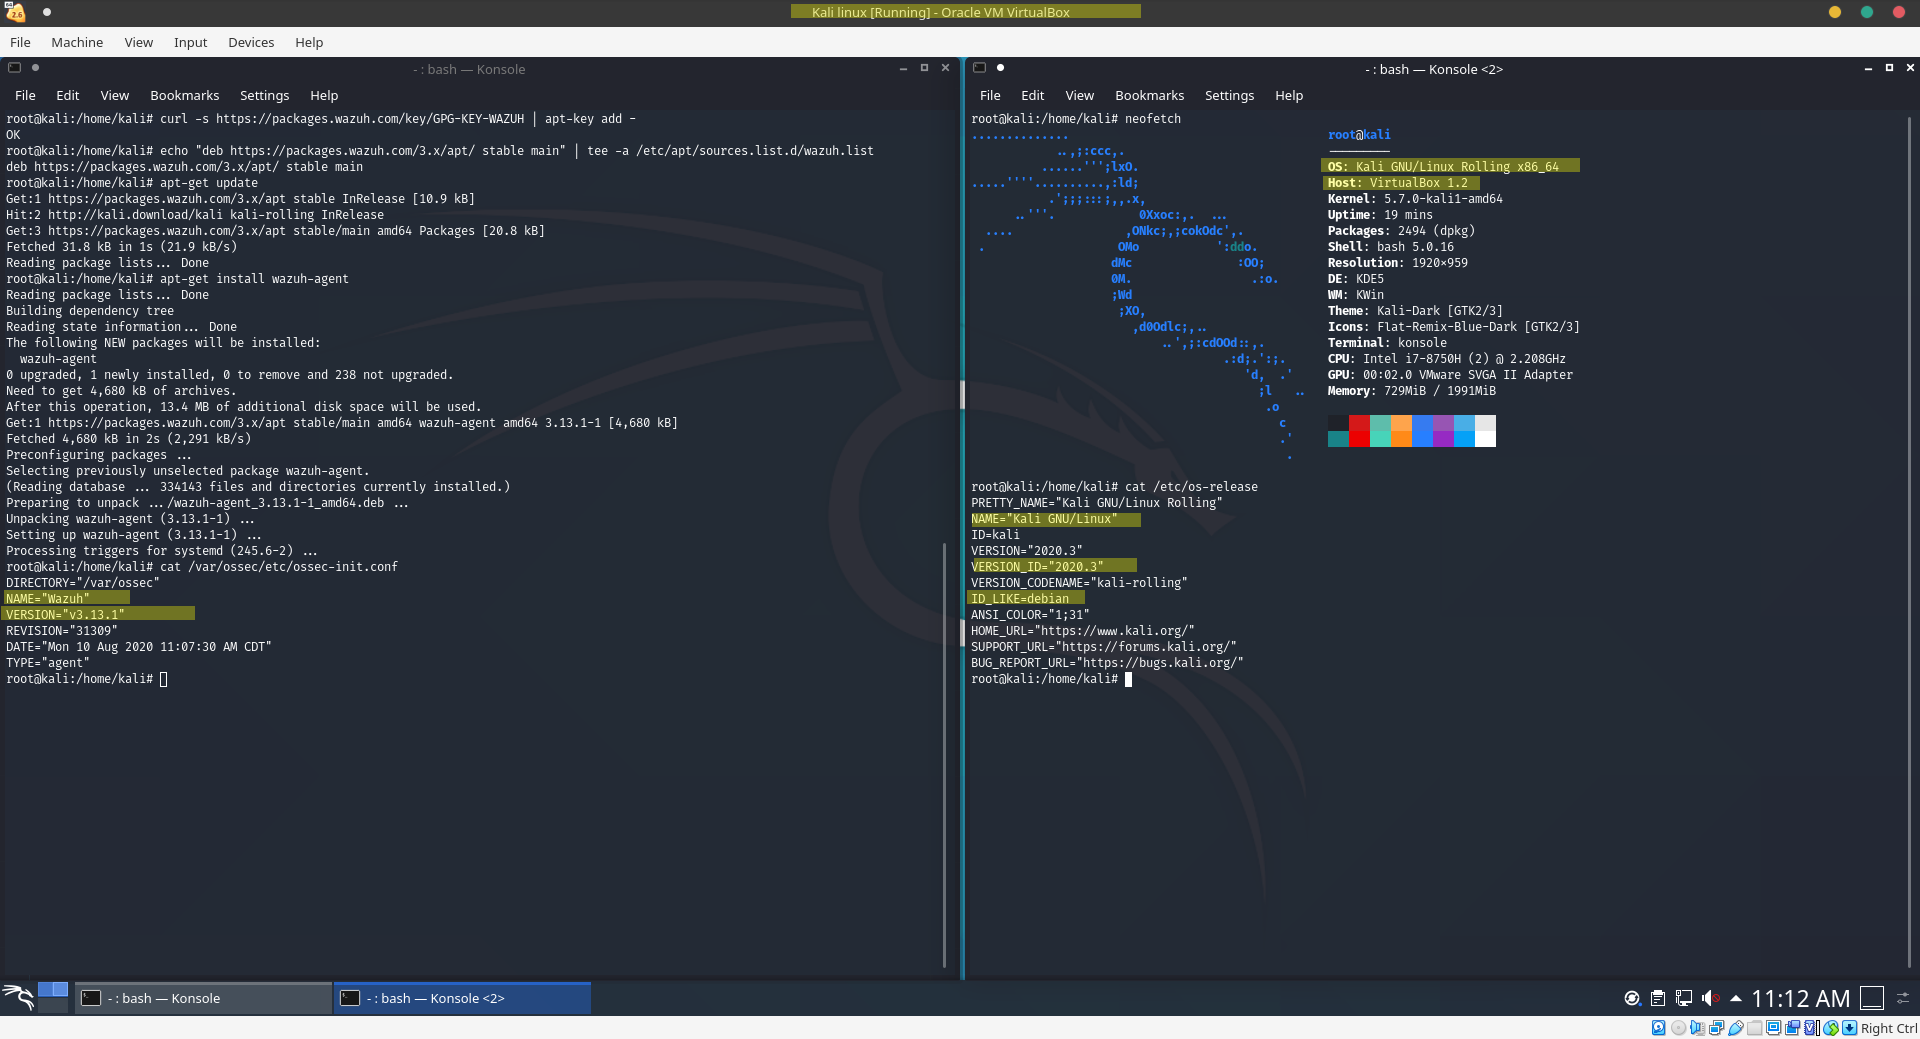
\includegraphics[width=\textwidth]{imagenes/kali_linux.png}
  \caption{Captura de pantalla del entorno virtualizado de Kali Linux mostrando alguna información del sistema y la instalación de Wazuh en varios terminales.}
  \label{kali1}
\end{figure}


Kali Linux es una \Gls{Rolling Release}, lo que significa que las actualizaciones se hacen de forma incremental y no tiene un versionado discreto. Para este estudio he utilizado una ISO etiquetada como \textbf{2020.04} (ver figura \ref{kali1} y la he instalado en una máquina virtual limpia. En el apartado siguiente discutiremos el uso de Wazuh en el proyecto y qué papel tendrá esta instancia desde la perspectiva de la arquitectura de Wazuh.

\subsection{Uso de Wazuh en Kali Linux}\label{sec:wazuh_kali}

Hemos hablado de varias formas de aprovechar Wazuh en una auditoría de seguridad. 

\begin{itemize}
    \item Por un lado, se podría \textbf{evaluar el rendimiento de la aplicación} ante un ataque simulado. Para ello, haría falta que el agente de Wazuh se encontrara instalado en la máquina que se va a evaluar y conectado a un Wazuh manager (preferiblemente instalado en otro dispositivo)  que además disponga de un servicio de Elasticsearch y Kibana.
    \item Por otro lado, queremos que Wazuh nos sirva para analizar y almacenar información extraída de los tests de penetración de sistemas. Para ello, necesitaríamos también dispone de un servidor de Wazuh manager de Wazuh (puede ser el mismo que para el caso anterior) junto con Elasticsearch y Kibana. Y necesitaremos otro agente de Wazuh instalado en la máquina `atacante' (Kali Linux) para recoger los datos generados durante la auditoría.
\end{itemize}

Una pregunta interesante sería si \textbf{verdaderamente hace falta un agente de Wazuh instalado en la máquina con Kali Linux}. La respuesta es que no es estrictamente necesario: existen otras formas de enviar datos a un Wazuh manager \textbf{sin hacer uso de un agente}, por ejemplo, utilizando un servicio \textbf{syslog} y enviando logs en ese formato al manager.

Esta opción sería perfectamente válida y eliminaría la necesidad de instalar y servir el agente de Wazuh, pero supondría otra necesidad: la de instalar y configurar un agente de syslog que sea capaz de enviar los logs a Wazuh. Además, una importante \textbf{ventaja de utilizar un agente Wazuh} es que sus mensajes se envían comprimidos y \textbf{encriptados} por defecto, lo que asegura una comunicación segura y es preferible a una comunicación con formato syslog (cuya seguridad depende del software utilizado y de su configuración y en algunas ocasiones no se tiene lo suficientemente en cuenta).

Por otro lado: hay que distinguir un caso de uso posible similar al que se describió en la introducción al hablar sobre \textbf{Faraday}, que es el de usar Wazuh como un entorno colaborativo de pentesting, en el que un equipo de profesionales del sector podría conectarse a \textbf{un mismo manager} de forma que, teniendo todos acceso a la aplicación web de Kibana, pudieran compartir sus logs e información extraída durante una auditoría.

Si no es el caso, y solo existe un único profesional que vaya a realizar la auditoría, y si además la empresa no cuenta ya con un entorno con Wazuh y Elasticsearch configurado, otra opción que se puede valorar es la de \textbf{instalar directamente el Wazuh manager en Kali Linux} junto con Elasticsearch y Kibana, puesto que el propio manager también es capaz de recopilar información del sistema dónde se encuentra (como si fuera un agente) y así eliminaríamos comunicaciones y la necesidad de tener más de un servidor funcionando. Un ejemplo de la diferencia entre estas dos maneras de utilizar Wazuh se muestra en la figura  \ref{entorno_ejemplos}.

\begin{figure}[!hbt]
  \centering
  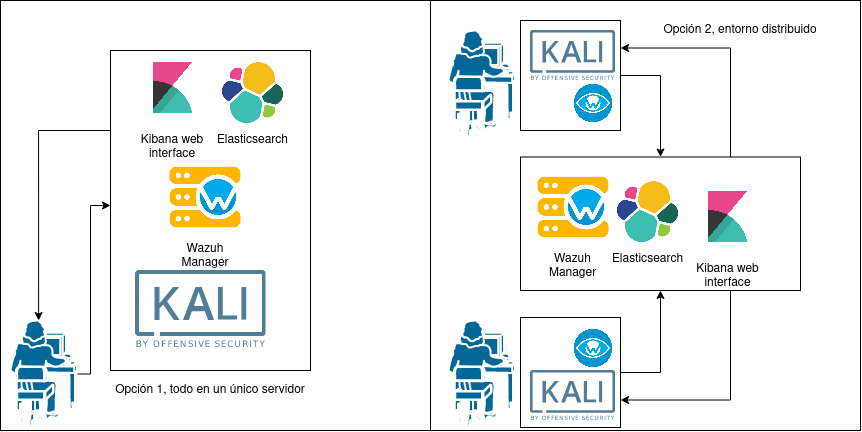
\includegraphics[width=\textwidth]{imagenes/entorno.png}
  \caption{Ejemplo de varias formas de distribuir los servicios para hacer uso de Wazuh. En la imagen de la izquierda se ve un entorno único, monousuario con todo instalado en una sola máquina y sin hacer uso de agentes, mientras que en la otra imagen se ve cómo podría distribuirse el entorno haciendo uso de agentes para ser utilizado por más de una persona.}
  \label{entorno_ejemplos}
\end{figure}


Para el trabajo se ha utilizado la opción de instalar un Mánager de Wazuh, así como el servicio de Elasticsearch y Kibana, todo en el mismo servidor con Kali Linux. Esto se ha llevado a cabo utilizando una máquina virtual, pero también podría realizarse por medio de Dockers, de forma que los distintos servicios se separaran por contenedores y se simplifica el despliegue de los mismos.

A este servidor se le conectará además un agente instalado en la máquina vulnerable que se estudiará en el caso práctico de la fase final.